\section{ShapeNet}

ShapeNet \cite{ChangFunkhouserGuibasSavarese:2015} is our first dataset
comprising realistic objects, in particular cars.
Later, ShapeNet will also be used to train the shape prior for shape
completion on KITTI \cite{GeigerLenzUrtasun:2012,GeigerLenzStillerUrtasun:2013}.
We first manually discarded
$262$ of the $3514$ simplified meshes that could not be automatically scale
and rotated to $[0,1]^3$ for further processing. We split the remaining models
into two training sets -- for prior and inference -- and a validation set
corresponding to the fractions $0.45:0.45:0.1$. On each model, we apply seven
random transformations including slight scaling, rotation and
translation to the meshes; additionally,
we flip every variant. Overall, we obtain the datasets outlined
in Table \ref{table:experiments-shapenet-datasets}; examples can be found
in Appendix \ref{ch:appendix-data}.

\begin{table}
  \centering
  {\footnotesize
  \renewcommand{\arraystretch}{1.1}
  \begin{tabularx}{\textwidth}{| X | c | c | c |}
    \hline
    & \Cub\easy & \Cub\moderate & \Cub\hard\\\hline
    Training Size (Prior/Inference) & \multicolumn{3}{c|}{$20496/20496$}\\\hline
    Validation Size & \multicolumn{3}{c|}{$4550$}\\\hline
    Resolution $H \times W \times D$ & \multicolumn{3}{c|}{$32 \times 32 \times 32$}\\\hline
    Resolution $2u \times 2v$ & $48 \times 64$ & \multicolumn{2}{c|}{$24 \times 32$}\\\hline
    Noise $\lambda_{\text{hit}}$ & $0$ & $50$ & $50$\\\hline
    Noise $\theta_{\text{ignore}}$ & $0$ & $0$ & $0.075$\\\hline
    Observed Voxels & $0.62\%$ & $0.31\%$ & $0.304\%$\\\hline
    Free Space Voxels & $3.91\%$ & $3.75\%$ & $4.37\%$\\\hline
    Observed Voxels & $5.54\%$ & $5.51\%$ & $5.52\%$\\\hline
  \end{tabularx}
  }
  \vskip 6px
  % TODO short caption
  \caption{Overview of the generated datasets. We created datasets of three
  difficulties, \easy, \moderate and \hard, which refer to increased noise
  and less observations. Details on the parameters are discussed
  in Section \ref{sec:data-3d}.}
  \label{table:experiments-shapenet-datasets}
\end{table}

\subsection{Shape Prior}

\begin{figure}[b]
  \centering
  \begin{subfigure}[t]{0.48\textwidth}
    \begin{tikzpicture}
      \begin{axis}[
          % https://tex.stackexchange.com/questions/68577/compiling-a-document-with-pgfplots-processing-only-every-x-th-data-point
          each nth point=4,
          filter discard warning=false,
          unbounded coords=discard,
          % https://tex.stackexchange.com/questions/13816/dimension-too-large-while-plotting-with-pgfplots
          %restrict y to domain=0:0.1,
          %restrict x to domain=0:250000,
          log ticks with fixed point,
          ymin=0,
          ymax=0.05,
          xmin=0,
          xmax=250000,
          %xticklabel={
          %  \pgfmathparse{\tick/1000}
          %  \pgfmathprintnumber{\pgfmathresult}k
          %},
          xtick={0,50000,100000,150000,200000,250000},
          xticklabels={0,50k,100k,150k,200k,250k},
          xticklabel style={
            /pgf/number format/fixed
          },
          scaled x ticks=false,
          yticklabel style={
            /pgf/number format/fixed
          },
          scaled y ticks=false,
          %x coord trafo/.code={\pgfmathparse{\pgfmathresult/1000}},
          %xticklabel=\pgfmathprintnumber{\tick}k,
          width=7.5cm,
          height=5cm,
          % https://tex.stackexchange.com/questions/48620/pgfplots-alignment-and-size-of-math-in-legend
          legend cell align=left,
        ]
        
        % https://tex.stackexchange.com/questions/276869/reading-an-unusual-coordinates-file-in-pgfplots
        \addplot +[mark=none] table[ignore chars={(,)},col sep=comma] {data/experiments/shapenet/vae_occ/easy_15_long/training_loss.txt};
        \addlegendentry{$\mathcal{L}_{\text{BCE}} + \KL$ (train)};
        \addplot +[mark=none] table[ignore chars={(,)},col sep=comma] {data/experiments/shapenet/vae_occ/easy_15_long/training_abs.txt};
        \addlegendentry{$\Abs$ (train)};
        
        \addplot +[mark=none] table[ignore chars={(,)},col sep=comma] {data/experiments/shapenet/vae_occ/easy_15_long/validation_loss.txt};
        \addlegendentry{$\mathcal{L}_{\text{BCE}} + \KL$ (val)};
        \addplot +[mark=none] table[ignore chars={(,)},col sep=comma] {data/experiments/shapenet/vae_occ/easy_15_long/validation_abs.txt};
        \addlegendentry{$\Abs$ (val)};
      \end{axis}
    \end{tikzpicture}
  \end{subfigure}\hfill
  \begin{subfigure}[t]{0.48\textwidth}
    \begin{tikzpicture}
      \begin{axis}[
          % https://tex.stackexchange.com/questions/68577/compiling-a-document-with-pgfplots-processing-only-every-x-th-data-point
          each nth point=2,
          filter discard warning=false,
          unbounded coords=discard,
          % https://tex.stackexchange.com/questions/13816/dimension-too-large-while-plotting-with-pgfplots
          %restrict y to domain=0:0.1,
          %restrict x to domain=0:250000,
          %ymin=0,
          ymax=0.5,
          xmin=0,
          xmax=250000,
          %xticklabel={
          %  \pgfmathparse{\tick/1000}
          %  \pgfmathprintnumber{\pgfmathresult}k
          %},
          xtick={0,50000,100000,150000,200000,250000},
          xticklabels={0,50k,100k,150k,200k,250k},
          xticklabel style={
            /pgf/number format/fixed
          },
          scaled x ticks=false,
          yticklabel style={
            /pgf/number format/fixed
          },
          scaled y ticks=false,
          %x coord trafo/.code={\pgfmathparse{\pgfmathresult/1000}},
          %xticklabel=\pgfmathprintnumber{\tick}k,
          width=7.5cm,
          height=5cm,
          % https://tex.stackexchange.com/questions/48620/pgfplots-alignment-and-size-of-math-in-legend
          legend cell align=left,
        ]
        
        \addplot +[mark=none] table[ignore chars={(,)},col sep=comma] {data/experiments/shapenet/vae_occ/easy_15_long/validation_mean.txt};
        \addlegendentry{$\overline{\mu}$ (val)};
        \addplot +[mark=none] table[ignore chars={(,)},col sep=comma] {data/experiments/shapenet/vae_occ/easy_15_long/validation_var.txt};
        \addlegendentry{$\exp\left(\frac{1}{2}\overline{l}\right)$ (val)};
        \addplot +[mark=none] table[ignore chars={(,)},col sep=comma] {data/experiments/shapenet/vae_occ/easy_15_long/validation_std.txt};
        \addlegendentry{$|1 - \sqrt{\Var[\mu]}|$ (val)};
      \end{axis}
    \end{tikzpicture}
  \end{subfigure}
  \vskip 6px
  
  % TODO short caption
  \caption{Training curves for a \VAE with $Q = 15$ trained on occupancy only
  on the ShapeNet dataset. In comparison with Figure \ref{fig:experiments-3d-vae-t},
  we plot training (train) and validation (val) loss, \ie $\mathcal{L}_{\text{BCE}} + \KL$,
  the corresponding absolute error \Abs as well as latent space statistics
  $\overline{\mu}$, $\sqrt{\Var[\mu]}$ and $\exp(\frac{1}{2} \overline{l})$
  corresponding to the average of the precited means, the corresponding standard
  deviation and the average of the predicted standard deviations.}
  \label{fig:experiments-shapenet-vae-t}
\end{figure}

% TODO replace by long version
\begin{figure}
  \centering
  \begin{tikzpicture}    
    %\node at (-3.5,0) {
    %  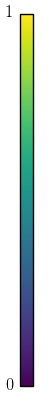
\includegraphics[height=5cm]{experiments/3d/vae_occ_sdf/colorbar_0}
    %};
    
    \node at (0, 1.2){
      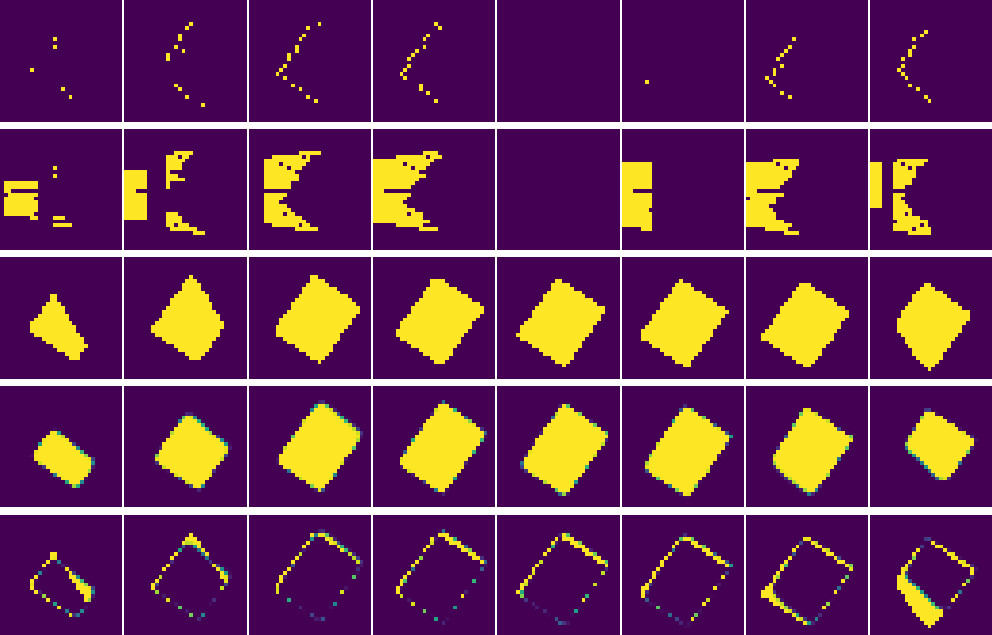
\includegraphics[width=6cm]{experiments/shapenet/vae_occ/easy_15_long/results_1}
    };
    \node at (0, -1.2){
      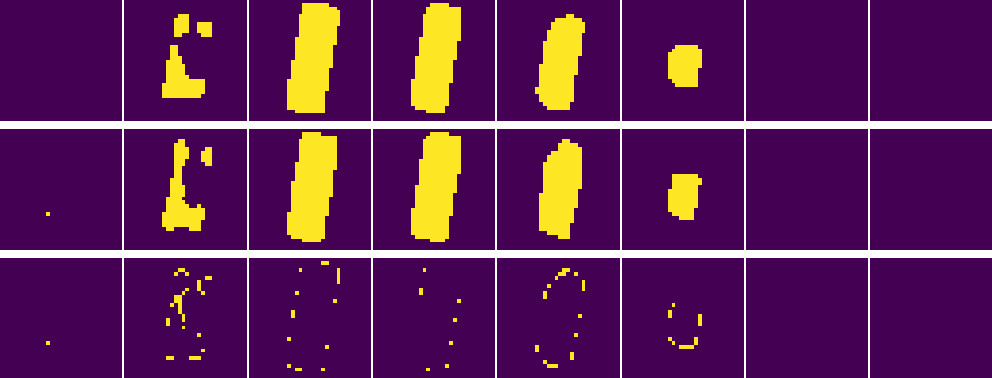
\includegraphics[width=6cm]{experiments/shapenet/vae_occ/easy_15_long/results_2}
    };
    
    \node at (6.5, 0){
      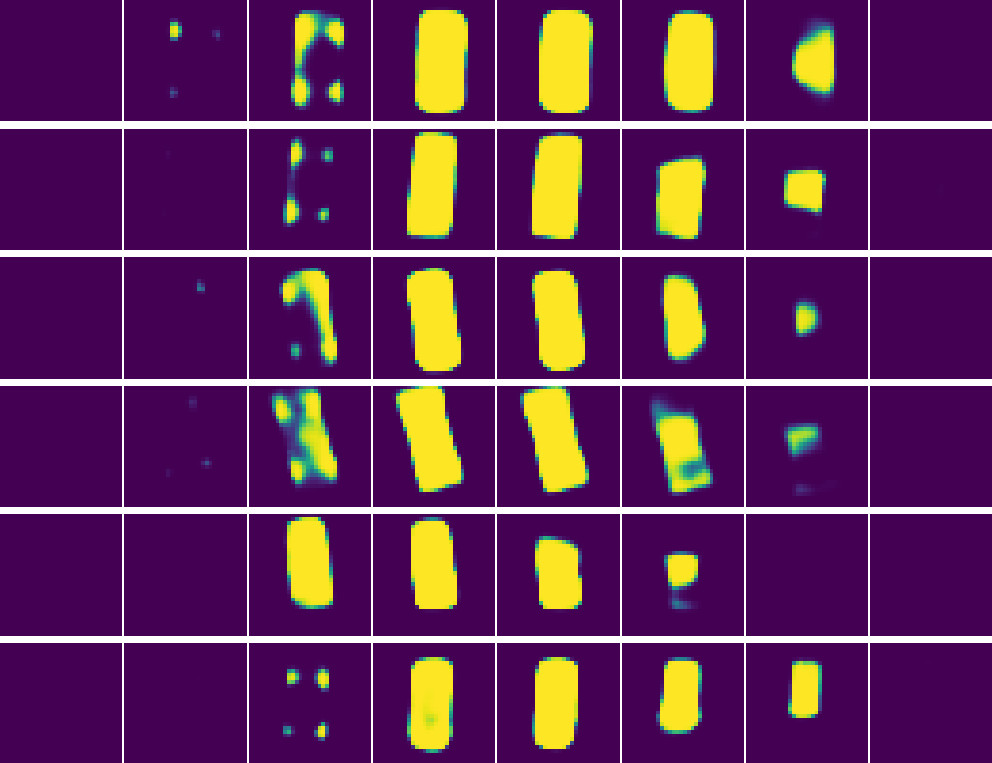
\includegraphics[width=6cm]{experiments/shapenet/vae_occ/easy_15_long/random_0}
    };
    
    \node at (0, 3) {\begin{tabular}{c}reconstruction\\occupancy\end{tabular}};
    \node at (6.5, 3) {\begin{tabular}{c}random samples\\occupancy\end{tabular}};
    
    \draw[-,dashed] (-3.5, -2.5) -- (10, -2.5);
    
    \node at (10, 0) {
      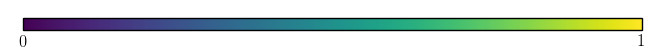
\includegraphics[height=4.2cm]{experiments/3d/vae_occ/easy_15/colorbar}
    };
    
    %\node at (-3.5,-5) {
    %  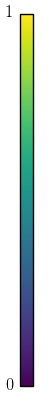
\includegraphics[height=5cm]{experiments/3d/vae_occ_sdf/colorbar_0}
    %};
    
    \node at (0, -5){
      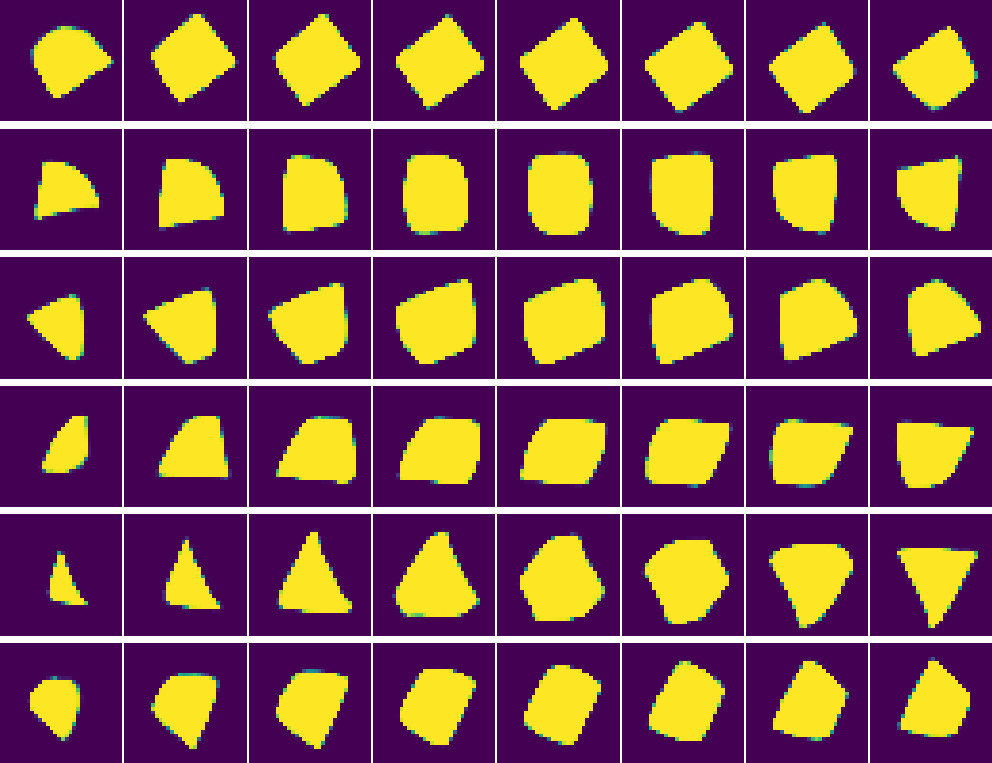
\includegraphics[width=6cm]{experiments/shapenet/vae_occ_sdf/easy_15/random_0_0}
    };
    
    %\draw[-,dashed] (3.25, -3) -- (3.25,3);
    
    \node at (6.5, -5){
      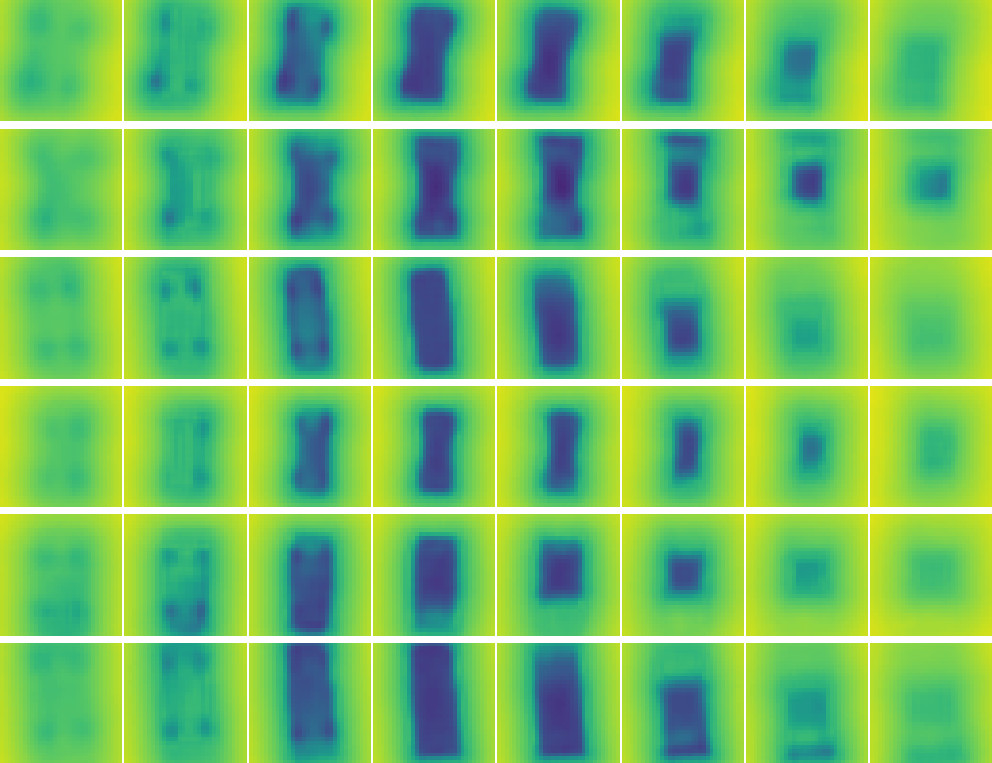
\includegraphics[width=6cm]{experiments/shapenet/vae_occ_sdf/easy_15/random_0_1}
    };
    
    \node at (10,-5) {
      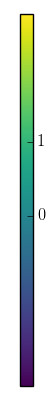
\includegraphics[height=5cm]{experiments/3d/vae_occ_sdf/colorbar_1}
    };
    
    \node[rotate=90] at (-3.75, 0) {\begin{tabular}{c}predicting occupancy only\end{tabular}};
    \node[rotate=90] at (-3.75, -5) {\begin{tabular}{c}predicting occupancy and\\signed distance functions\end{tabular}};
        
    \node at (0, -8) {\begin{tabular}{c}random samples\\occupancy\end{tabular}};
    \node at (6.5, -8) {\begin{tabular}{c}random samples\\signed distance functions\end{tabular}};
  \end{tikzpicture}
  \caption{Qualitative results considering reconstruction and random samples
  for a \VAE prior, $Q = 15$, learned on ShapeNet using occupancy only (top) and
  both occupancy and signed distance functions. In the latter case we only show
  random samples in both modalities. For reconstructions we show the target shape,
  the prediction as well as the corresponding error. In all cases we resort to
  showing horizontal slices as done before. 3D visualizations
  of the random samples can be found in Figures \ref{fig:experiments-shapenet-vae-qual-2}
  and \ref{fig:experiments-shapenet-vae-qual-3}.}
  \label{fig:experiments-shapenet-vae-qual-1}
\end{figure}
\begin{figure}
  \centering
  \hspace*{-0.75cm}
  \begin{tikzpicture}
    \node at (0, 0) {
      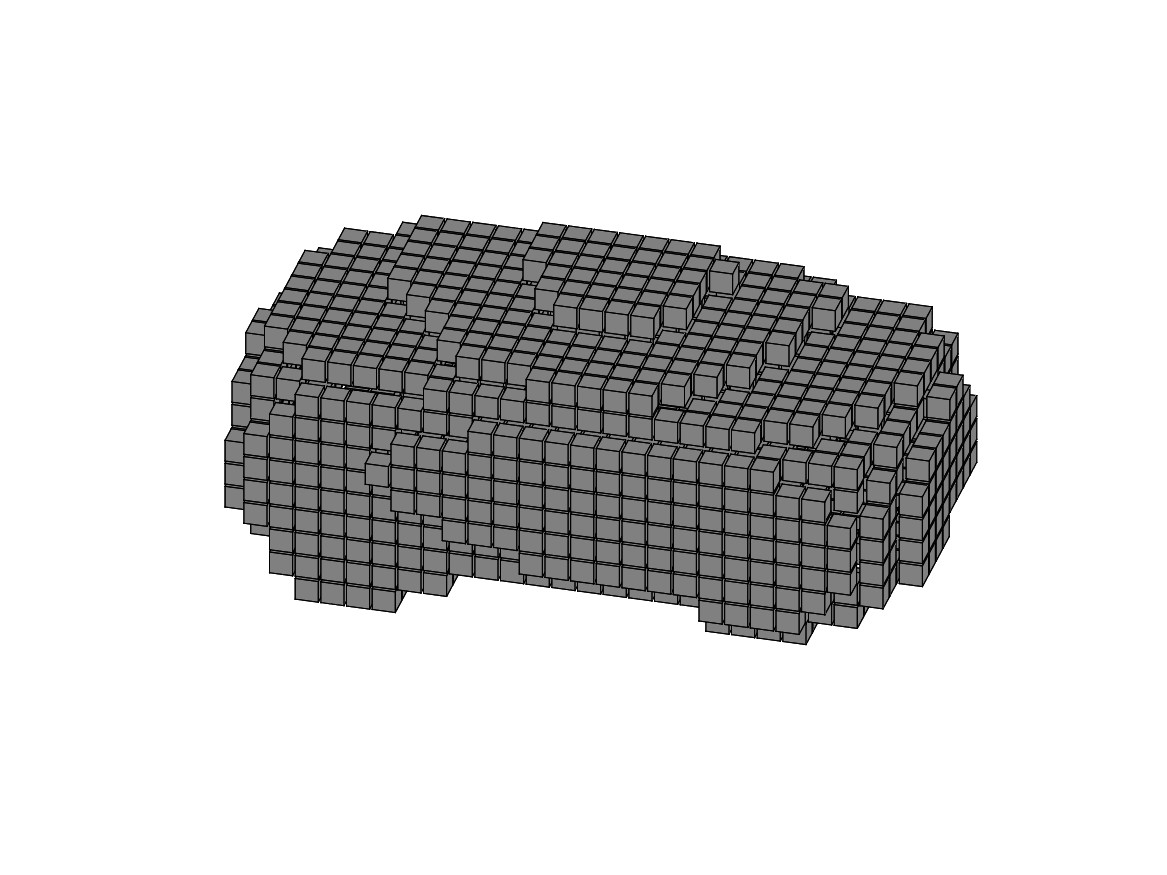
\includegraphics[width=2.5cm,trim={2cm 1cm 2cm 1cm},clip]{experiments/shapenet/vae_occ/easy_15_long/0_random_15}
    };
    \node at (2.5, 0) {
      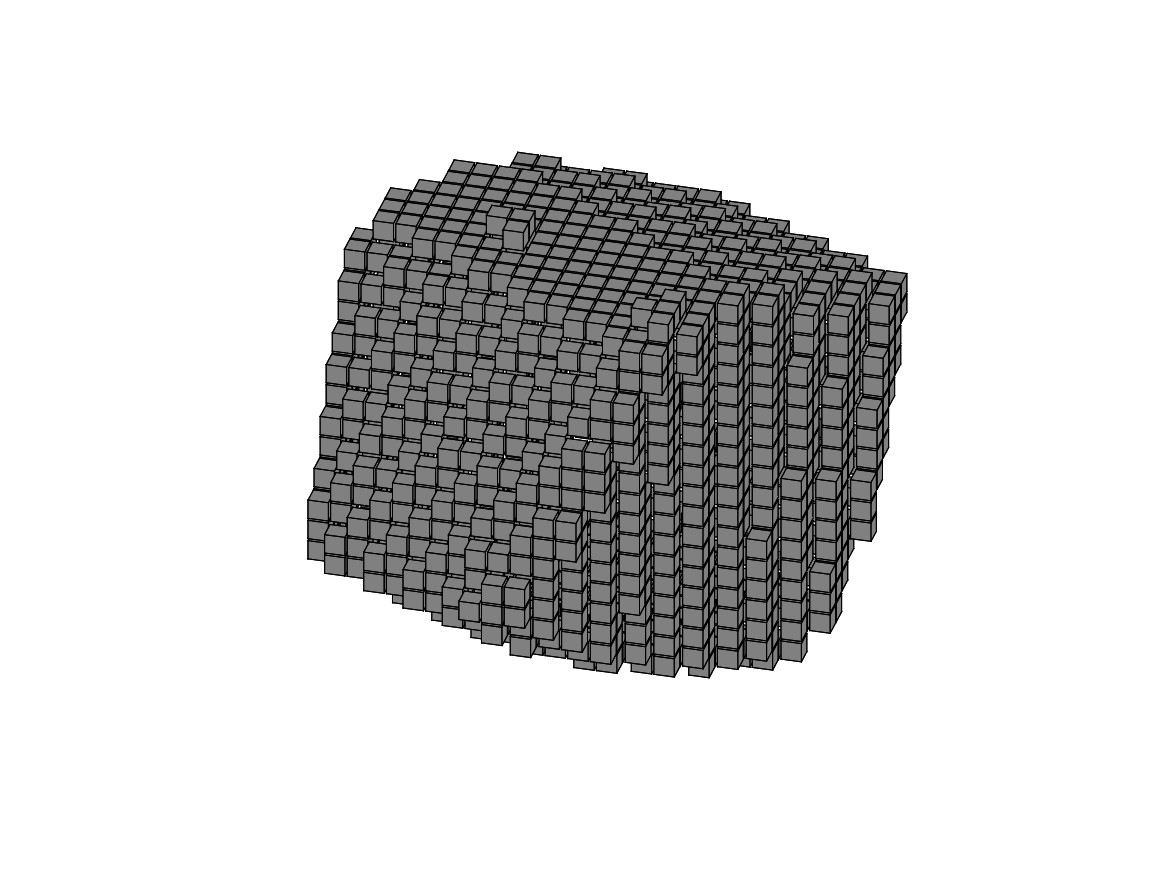
\includegraphics[width=2.5cm,trim={2cm 1cm 2cm 1cm},clip]{experiments/shapenet/vae_occ/easy_15_long/0_random_105}
    };
    
    \draw[-,dashed] (4,-1.5) -- (4, 1.5);
    
    \node at (5.5, 0) {
      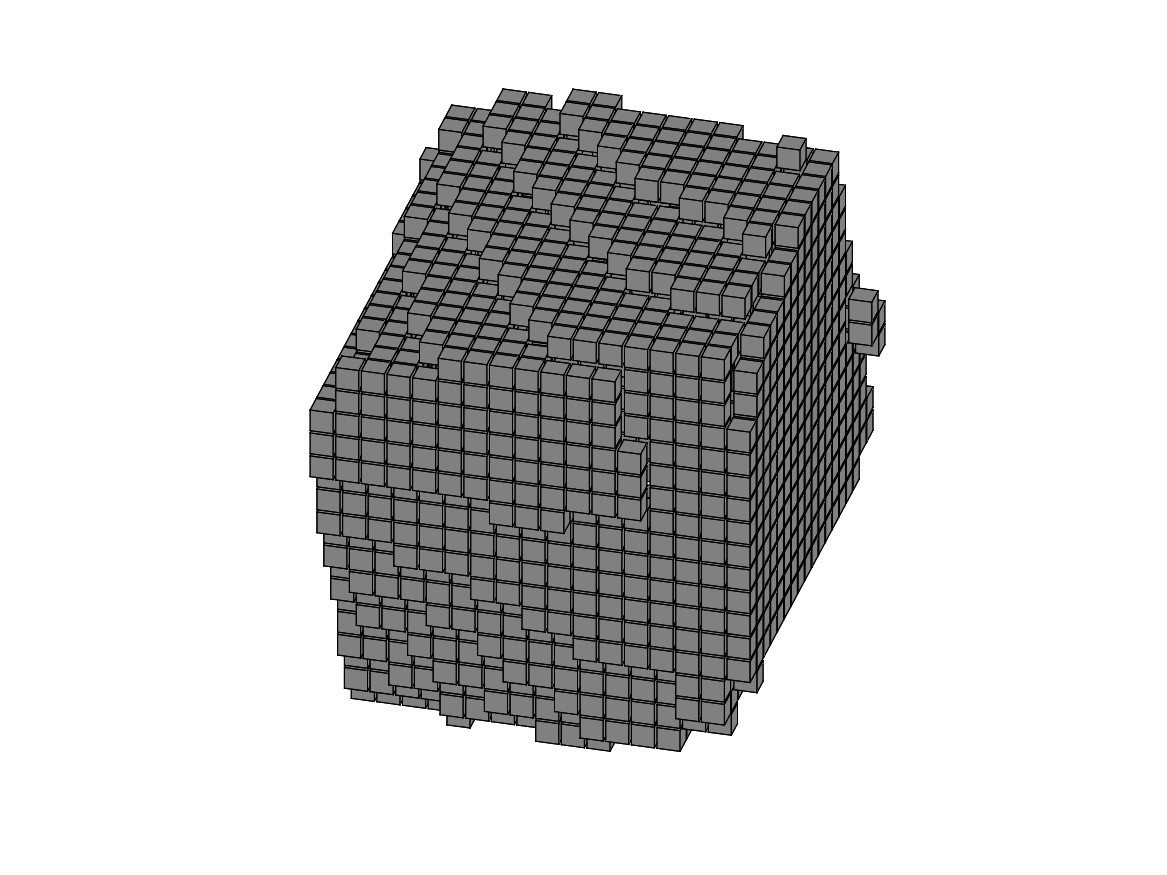
\includegraphics[width=2.5cm,trim={2cm 1cm 2cm 1cm},clip]{experiments/shapenet/vae_occ/easy_15_long/5_random_15}
    };
    \node at (8, 0) {
      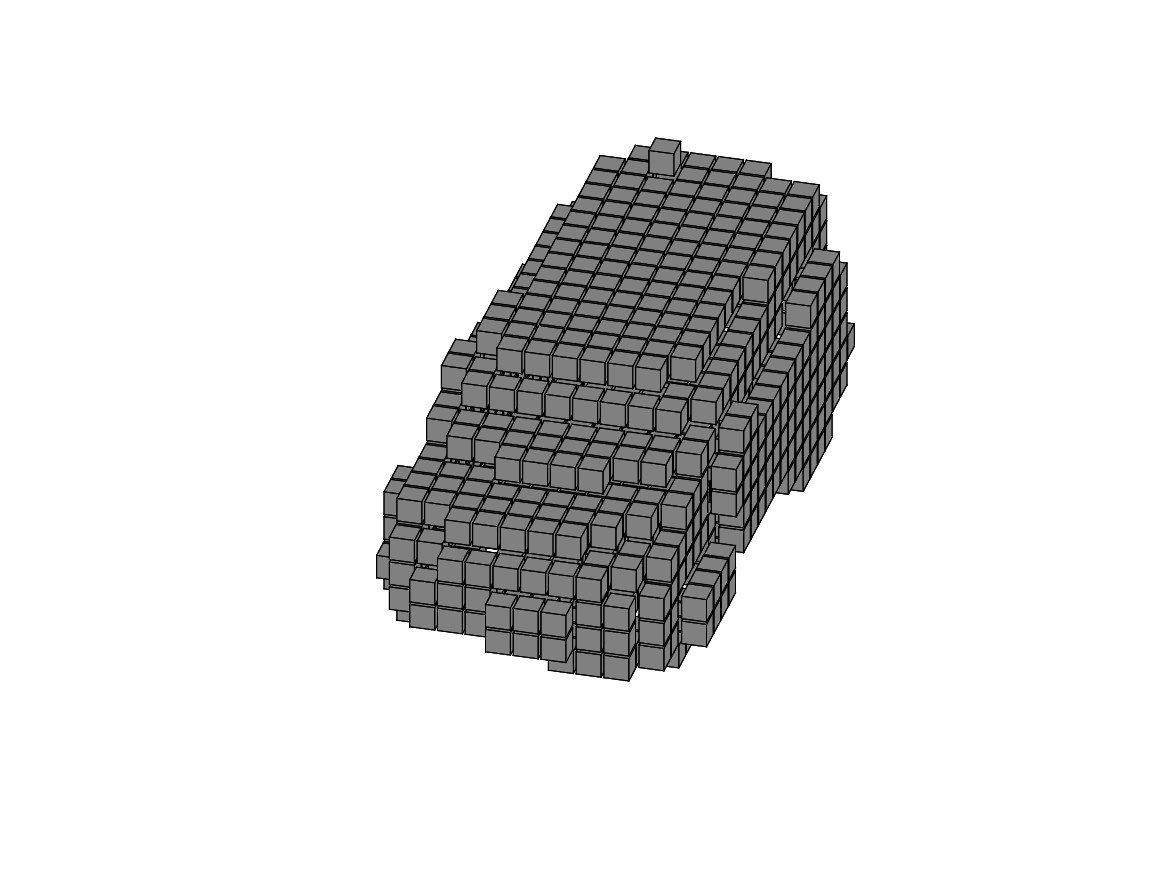
\includegraphics[width=2.5cm,trim={2cm 1cm 2cm 1cm},clip]{experiments/shapenet/vae_occ/easy_15_long/5_random_105}
    };
    
    \draw[-,dashed] (9.5,-1.5) -- (9.5, 1.5);
    
    \node at (11, 0) {
      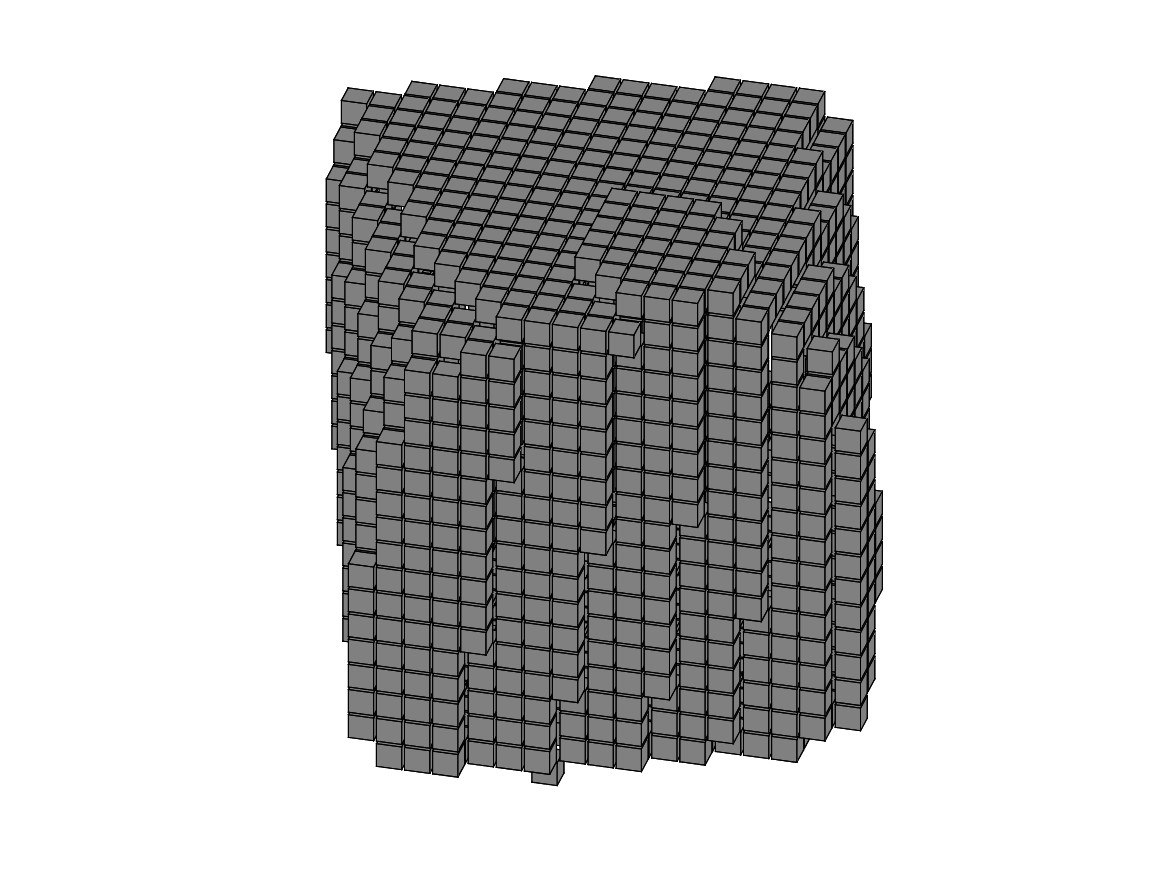
\includegraphics[width=2.5cm,trim={2cm 1cm 2cm 1cm},clip]{experiments/shapenet/vae_occ/easy_15_long/2_random_15}
    };
    \node at (13.5, 0) {
      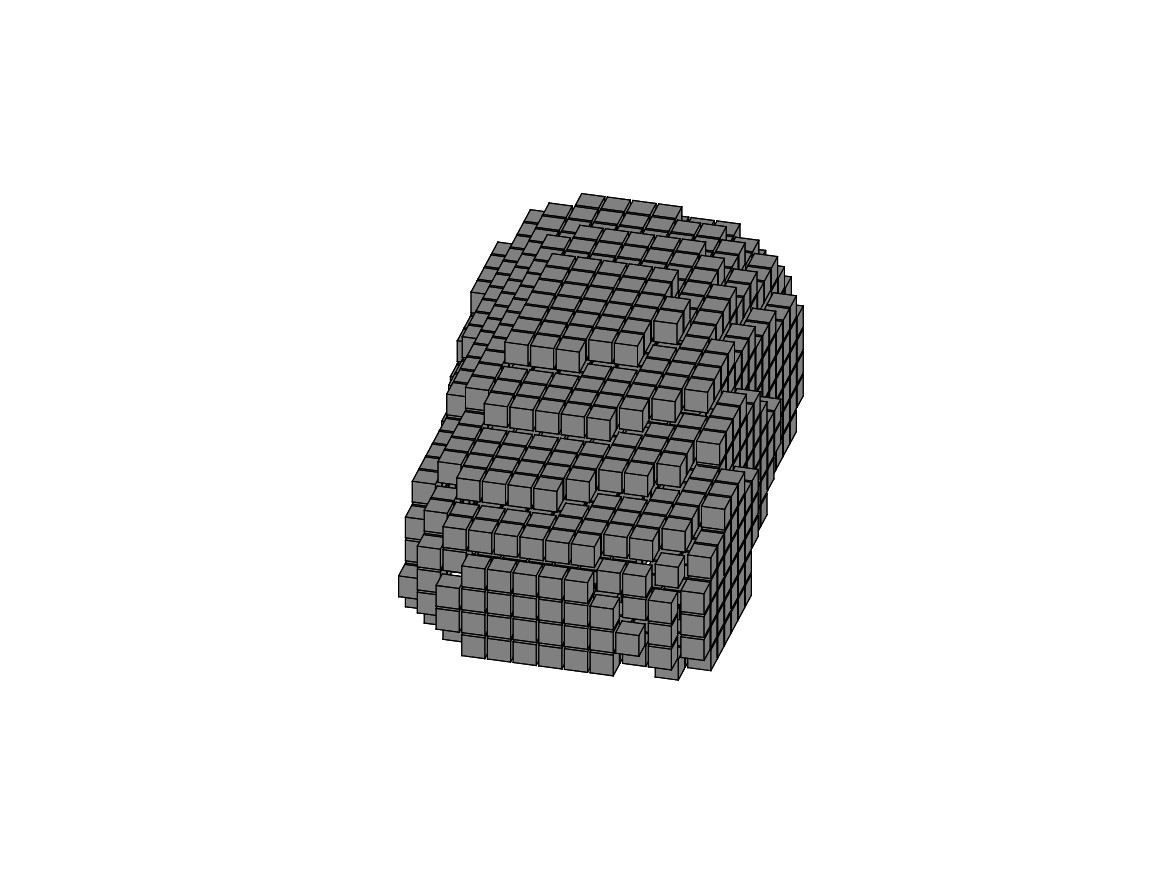
\includegraphics[width=2.5cm,trim={2cm 1cm 2cm 1cm},clip]{experiments/shapenet/vae_occ/easy_15_long/2_random_105}
    };
  \end{tikzpicture}
  \caption{3D visualizations of random samples obtained from a \VAE prior
  trained with $Q = 15$ and occupancy only on the ShapeNet dataset. We show three
  distinct samples using two viewpoints each. The samples
  can easily be recognized as cars, although details seem to be missing. However,
  this is also due to the low resolution of $32^3$ used.}
  \label{fig:experiments-shapenet-vae-qual-2}
\end{figure}
\begin{figure}
  \centering
  \hspace*{-0.5cm}
  \begin{tikzpicture}   
    \node at (0, 0) {
      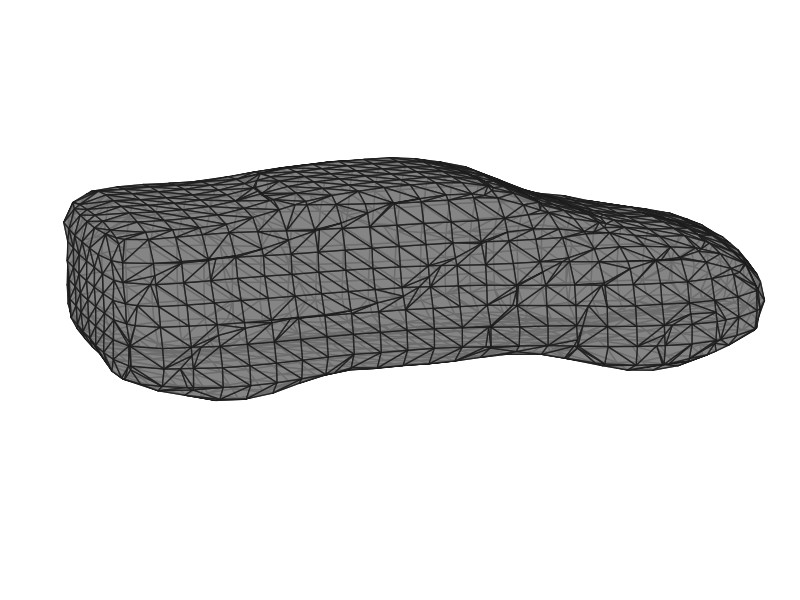
\includegraphics[width=2.4cm,trim={1cm 3cm 1cm 3cm},clip]{experiments/shapenet/vae_occ_sdf/easy_15/0_random}
    };
    
    \draw[-,dashed] (1.25,-1) -- (1.25, 1);
    
    \node at (2.5, 0) {
      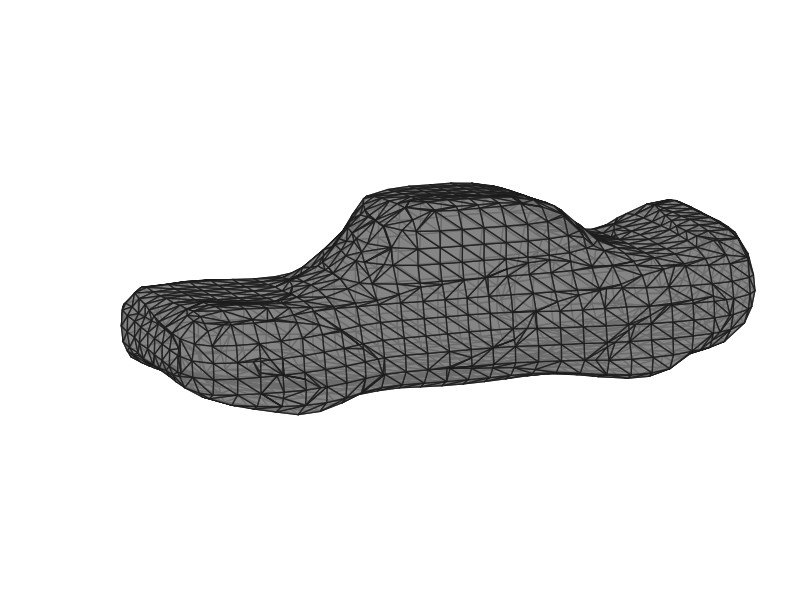
\includegraphics[width=2.4cm,trim={1cm 3cm 1cm 3cm},clip]{experiments/shapenet/vae_occ_sdf/easy_15/1_random}
    };
    
    \draw[-,dashed] (3.75,-1) -- (3.75, 1);
    
    \node at (5, 0) {
      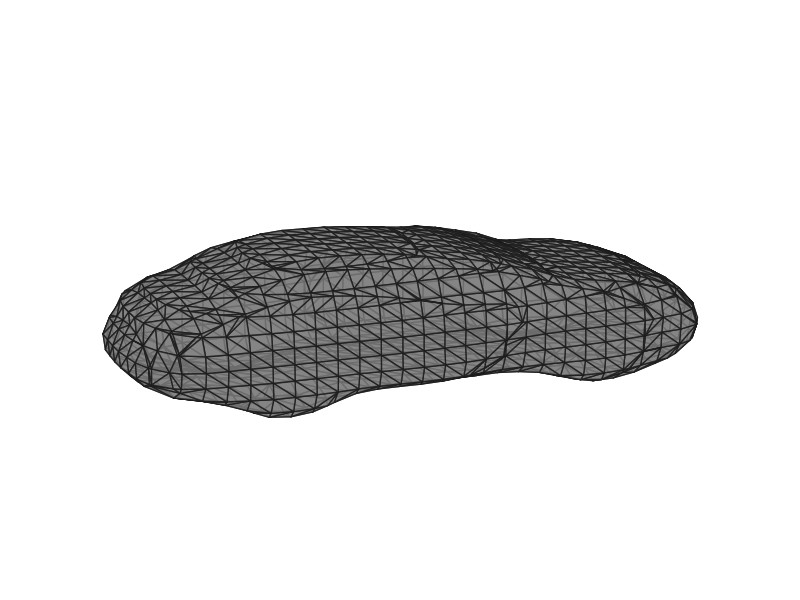
\includegraphics[width=2.4cm,trim={1cm 3cm 1cm 3cm},clip]{experiments/shapenet/vae_occ_sdf/easy_15/2_random}
    };
    
    \draw[-,dashed] (6.25,-1) -- (6.25, 1);
    
    \node at (7.5, 0) {
      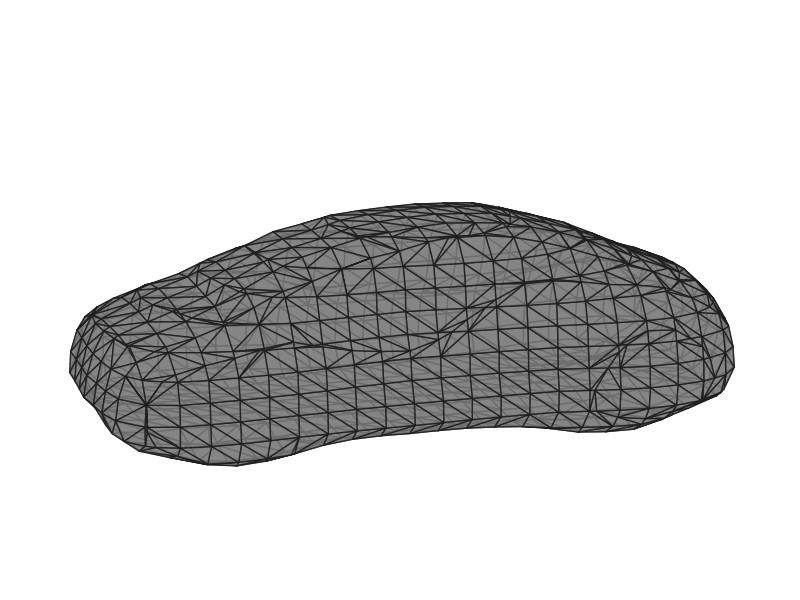
\includegraphics[width=2.4cm,trim={1cm 3cm 1cm 3cm},clip]{experiments/shapenet/vae_occ_sdf/easy_15/3_random}
    };
    
    \draw[-,dashed] (8.75,-1) -- (8.75, 1);
    
    \node at (10, 0) {
      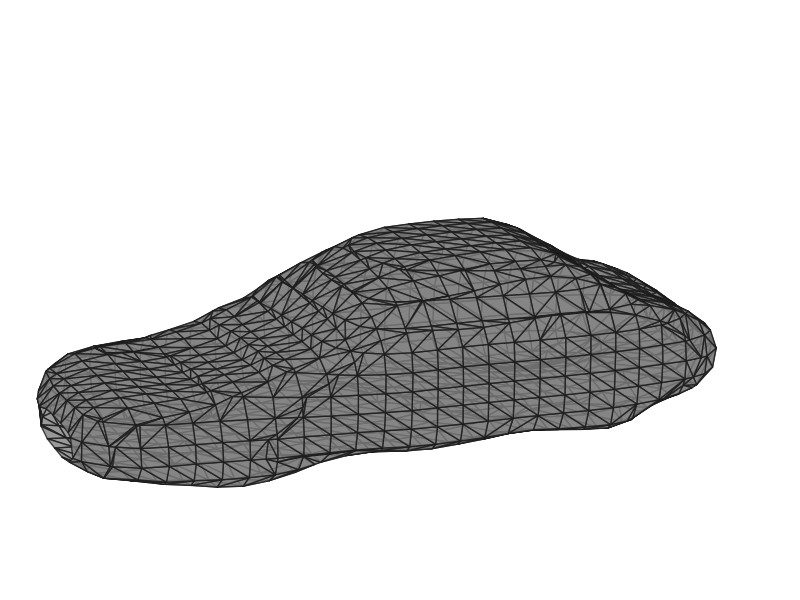
\includegraphics[width=2.4cm,trim={1cm 3cm 1cm 3cm},clip]{experiments/shapenet/vae_occ_sdf/easy_15/4_random}
    };
    
    \draw[-,dashed] (11.25,-1) -- (11.25, 1);
    
    \node at (12.5, 0) {
      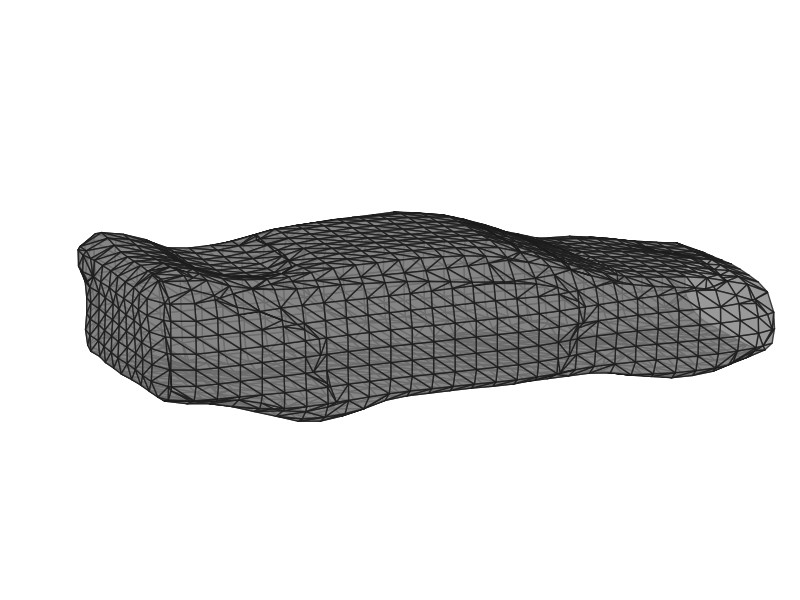
\includegraphics[width=2.4cm,trim={1cm 3cm 1cm 3cm},clip]{experiments/shapenet/vae_occ_sdf/easy_15/5_random}
    };
  \end{tikzpicture}
  \caption{3D visualizations of meshed random samples from a \VAE trained
  on both occupancy and signed distance functions. For meshing, we used the marching
  cubes algorithm on the predicted signed distance functions. We show a single viewpoint
  for each sample.}
  \label{fig:experiments-shapenet-vae-qual-3}
\end{figure}


For the \VAE prior, we again use $Q = 15$.
From training, we might conclude that the
ShapeNet dataset is slightly easier to learn. In particular, considering
Figure \ref{fig:experiments-shapenet-vae-t} we notice that both reconstruction
and the latent space are learned faster. However, it is hard to say whether
ShapeNet is inherently easier than the 3D cuboids dataset. On the one hand, we
only consider slight rotations around all axes; on the other hand,
the cars show more intra-class variation compared to cuboids. Overall,
the model achieves an absolute error of $\Abs \approx 0.0073$ and
$\AbsThr \approx 0.0048$ after thresholding.
However, we note
that only $\sim 5.54\%$ of the voxels are occupied in the first place
(\cf Table \ref{table:experiments-shapenet-datasets}).
We also notice that the model is less certain considering the random
samples in Figures \ref{fig:experiments-shapenet-vae-qual-1}
and \ref{fig:experiments-shapenet-vae-qual-2}, \ie predictions
appear less sharp. Especially regarding the wheels and the roofs, the model
has difficulties. Overall, we are satisfied by the obtained performance --
for experiments on KITTI, we will also have more training data.

On ShapeNet, too, we trained a prior model on both occupancy and signed
distance functions. For the first time, we also demonstrate why
we would prefer to work with signed distance functions: it is possible
to derive triangular meshes at sub-voxel accuracy, \eg
using the marching cubes algorithm \cite{LorensenCline:1987}\footnote{
  We use the implementation by Pablo M\'{a}rquez Neila available at
  \url{https://github.com/pmneila/PyMCubes}.
}. Again, we use $Q = 15$ to achieve a thresholded absolute error $\AbsThr \approx 0.0048$
(occupancy) and $\AbsThr \approx 0.0053$ (signed distance function), respectively.
We show meshes corresponding to random samples in Figure
\ref{fig:experiments-shapenet-vae-qual-3}. In addition,
in Figure \ref{fig:experiments-shapenet-vae-qual-1},
we show both modalities, also to illustrate the involved uncertainty.
Overall, we find that the random samples are appropriate. While some random samples
appear rather weird, it is not hard to imagine that they depict cars.
We also want to stress that the meshes look rather smooth although the
signed distance functions the model was trained on were originally derived
from the occupancy grids. We assume this to be the result of the probabilistic
formulation, \ie of training a \VAE. In particular, the encoder predicts
a Gaussian distribution where all samples need to result in a proper reconstruction.
This forces the model the smoothly interpolate between shapes.

\subsection{Amortized Maximum Likelihood}

\begin{figure}
  \centering
  \begin{tikzpicture}
    \begin{axis}[
        ybar stacked,
        % https://tex.stackexchange.com/questions/119887/remove-the-scientific-notation-which-is-unreasonable
        yticklabel style={
          /pgf/number format/fixed,
          /pgf/number format/precision=5
        },
        scaled y ticks=false,
        %enlargelimits=0.15,
        legend style={
          at={(1.01,1)},
          anchor=north west,
        },
        % https://tex.stackexchange.com/questions/48620/pgfplots-alignment-and-size-of-math-in-legend
        legend cell align=left,
        xtick={
          1, 2,
          3, 4, 5,
          6, 7, 8,
          9, 10, 11,
          12
        },
        xticklabels={
          \VAE, \VAE +sdf,
          \AML\\\easy, \AML\\\moderate, \AML\\\hard,
          \EVAE\\\easy, \EVAE\\\moderate, \EVAE\\\hard,
          \AML +sdf\\\easy, \AML +sdf\\\moderate, \AML +sdf\\\hard,
          Baseline
        },
        x tick label style={text width=1.5cm,align=right},
        ymin=0,
        width=12.5cm,
        height=4cm,
        enlarge x limits=0.05,
        % https://tex.stackexchange.com/questions/271027/pgfplots-how-to-rotate-extra-x-tick-labels
        x tick label style={
          rotate=90,
          anchor=east,
        },
        %bar width=8,
      ]
      
      % AbsThr
      \addplot +[bar shift=-.2cm] coordinates {
        (1, 0.00505722)
        (2, 0.00475067)
        (3, 0.01667228)
        (4, 0.0215971)
        (5, 0.02619364)
        %
        (6, 0.02136223)
        (7, 0.02775098)
        (8, 0.03063716)
        %
        (9, 0.02538469)
        (10, 0.03168048)
        (11, 0.03483872)
        (12, 0.010504529630079)
      };
      \addlegendentry{\AbsThr (occ)}
      % Abs
      \addplot +[bar shift=-.2cm] coordinates {
        (1, 0.002275) % 0.00733222)
        (2, 0.00203) % 0.00678092)
        (3, 0.00101) % 0.01768816)
        (4, 0.00088) % 0.02247298)
        (5, 0.00099) % 0.02718333)
        %
        (6, 0.00083) % 0.02219768)
        (7, 0.00063) % 0.02838561)
        (8, 0.0031) % 0.03373657)
        %
        (9, 0.00051) % 0.02589711)
        (10, 0.00041) % 0.0320905)
        (11, 0.00019) % 0.0350219)
        (12, 0.003366) % 0.013873896760899)
      };
      \addlegendentry{\Abs (occ)}
      
      % -- 
      \resettwelvestackedplots
      
      % AbsThr
      \addplot +[bar shift=+.2cm] coordinates {
        (1, 0)
        (2, 0.00530342)
        (3, 0)
        (4, 0)
        (5, 0)
        %
        (6, 0)
        (7, 0)
        (8, 0)
        %
        (9, 0.02553955)
        (10, 0.03210551)
        (11, 0.03564795)
        (12, 0)
      };
      \addlegendentry{\AbsThr (sdf)}
      % Abs
      \addplot +[bar shift=+.2cm] coordinates {
        (1, 0)
        (2, 0.0733) % 0.07860103)
        (3, 0)
        (4, 0)
        (5, 0)
        %
        (6, 0)
        (7, 0)
        (8, 0)
        %
        (9, 0.15607) % 0.18164451)
        (10, 0.1978) % 0.2299151)
        (11, 0.2304) % 0.26641559)
        (12, 0)
      };
      \addlegendentry{\Abs (sdf)}
    \end{axis}
  \end{tikzpicture}
  
  % TODO short caption
  \caption{Absolute error \Abs and its thresholded variant \AbsThr,
  \ie the absolute error on thresholded predictions,
  comparing \AML and \EVAE with the supervised baseline and the
  reconstruction performance of the shape prior. For the \VAE shape prior,
  we report the reconstruction performance for training on
  occupancy only as well as on both occupancy and signed distance functions.
  For \AML, we also consider both modalities. For \EVAE and the supervised baseline,
  we present results on occupancy only. For the latter, we refer to
  Section \ref{sec:experiments-shapenet-supervised-baseline}
  for details. In all cases, the left bar represents
  results on occupancy; the right bar corresponds to results on signed distance
  functions (if applicable).}
  \label{fig:experiments-shapenet-aml-abs}
\end{figure}

\begin{figure}
  \centering
  \begin{tikzpicture}    
    \node at (10, 0) {
      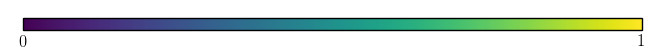
\includegraphics[height=4.2cm]{experiments/3d/vae_occ/easy_15/colorbar}
    };
    
    \node at (0, 0){
      \includegraphics[width=6cm]{experiments/shapenet/vae_occ_aml/hard_15_long_statistics_75/results_0}
    };
    
    \node at (6.5, 0){
      \includegraphics[width=6cm]{experiments/shapenet/vae_occ_aml/hard_15_long_statistics_75/results_3}
    };
    
    \draw[-,dashed](-3.5,-2.15) -- (10,-2.15);
    
    % --- 
    \node at (0, -3.5){
      \includegraphics[width=6cm]{experiments/shapenet/baseline/hard_15/results_0}
    };
    
    \node at (6.5, -3.5){
      \includegraphics[width=6cm]{experiments/shapenet/baseline/hard_15/results_3}
    };
    
    \node[rotate=90] at (-3.5, -3.5) {Baseline};
    \node[rotate=90] at (-3.5, 0) {\AML};
    %\node at (3.25, 2.5) {reconstruction};
  \end{tikzpicture}
  \vskip 6px
  
  % TODO short caption
  \caption{Qualitative results of \AML for \hard difficulty of the ShapeNet
  dataset. We show results for occupancy only in comparison with the supervised
  baseline. On top, we show horizontal slices of the volumes
  corresponding to the observed points, the partial free space, the target
  shape, the predicted shape and the corresponding error. On the bottom,
  \ie for the baseline, we only show the target shape, the predicted shape
  and the corresponding error. Again, we show heights $8 + 2i$ for
  $0 \leq i < 8$. 3D visualizations of these results can be found
  in Figure \ref{fig:experiments-shapenet-aml-qual-2}.}
  \label{fig:experiments-shapenet-aml-qual-1}
\end{figure}
\begin{figure}
  \centering
  \hspace*{-1cm}
  \begin{tikzpicture}
    \node at (0, 0) {
      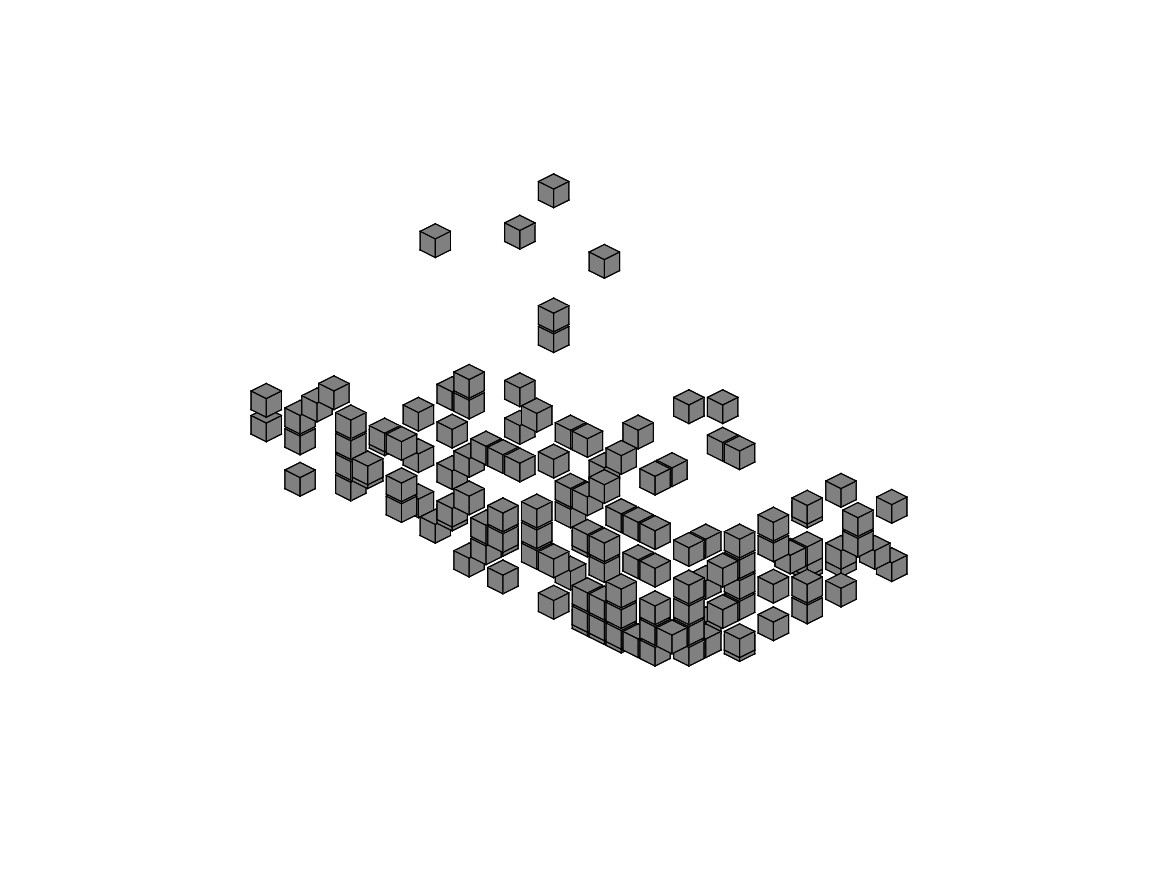
\includegraphics[width=3.75cm,trim={3.5cm 2.5cm 3.5cm 2.5cm},clip]{experiments/shapenet/vae_occ_aml/hard_15_long_statistics_75/0_input_45}
    };
    \node at (3.5, 0) {
      \includegraphics[width=3.75cm,trim={3.5cm 2.5cm 3.5cm 2.5cm},clip]{experiments/shapenet/vae_occ_aml/hard_15_long_statistics_75/0_prediction_45}
    };
    \node at (7, 0) {
      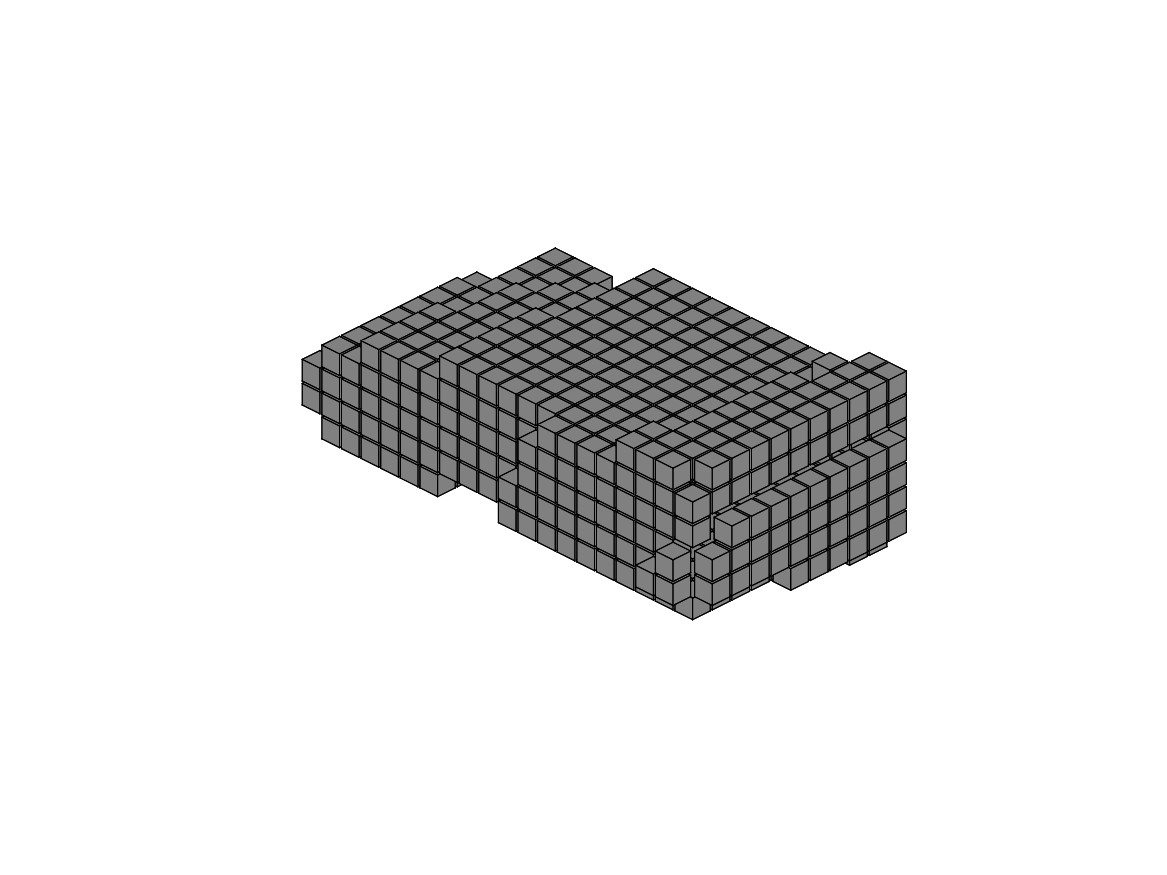
\includegraphics[width=3.75cm,trim={3.5cm 2.5cm 3.5cm 2.5cm},clip]{experiments/shapenet/vae_occ_aml/hard_15_long_statistics_75/0_target_45}
    };
    \node at (10.5, 0) {
      \includegraphics[width=3.75cm,trim={3.5cm 2.5cm 3.5cm 2.5cm},clip]{experiments/shapenet/baseline/hard_15/0_prediction_45}
    };
    
    \node at (0, -3) {
      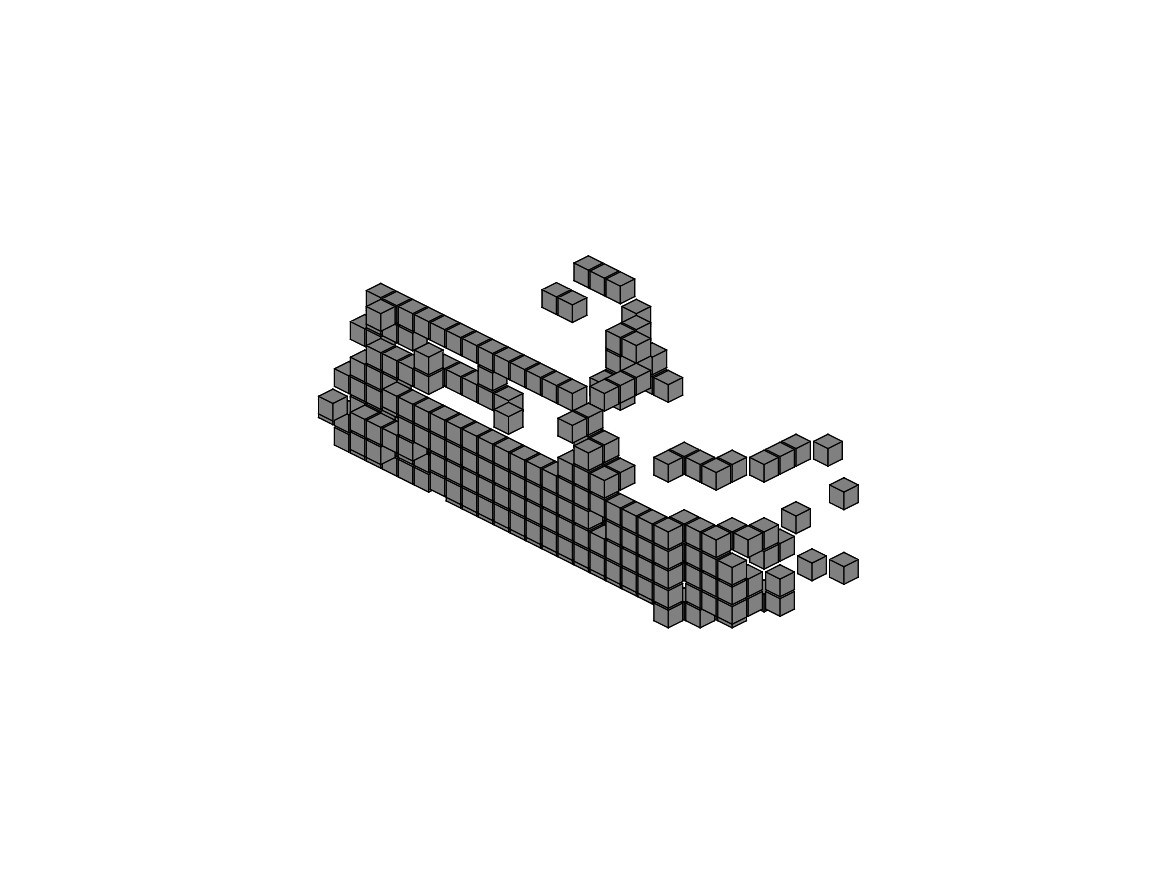
\includegraphics[width=3.75cm,trim={3.5cm 2.5cm 3.5cm 2.5cm},clip]{experiments/shapenet/vae_occ_aml/hard_15_long_statistics_75/3_input_45}
    };
    \node at (3.5, -3) {
      \includegraphics[width=3.75cm,trim={3.5cm 2.5cm 3.5cm 2.5cm},clip]{experiments/shapenet/vae_occ_aml/hard_15_long_statistics_75/3_prediction_45}
    };
    \node at (7, -3) {
      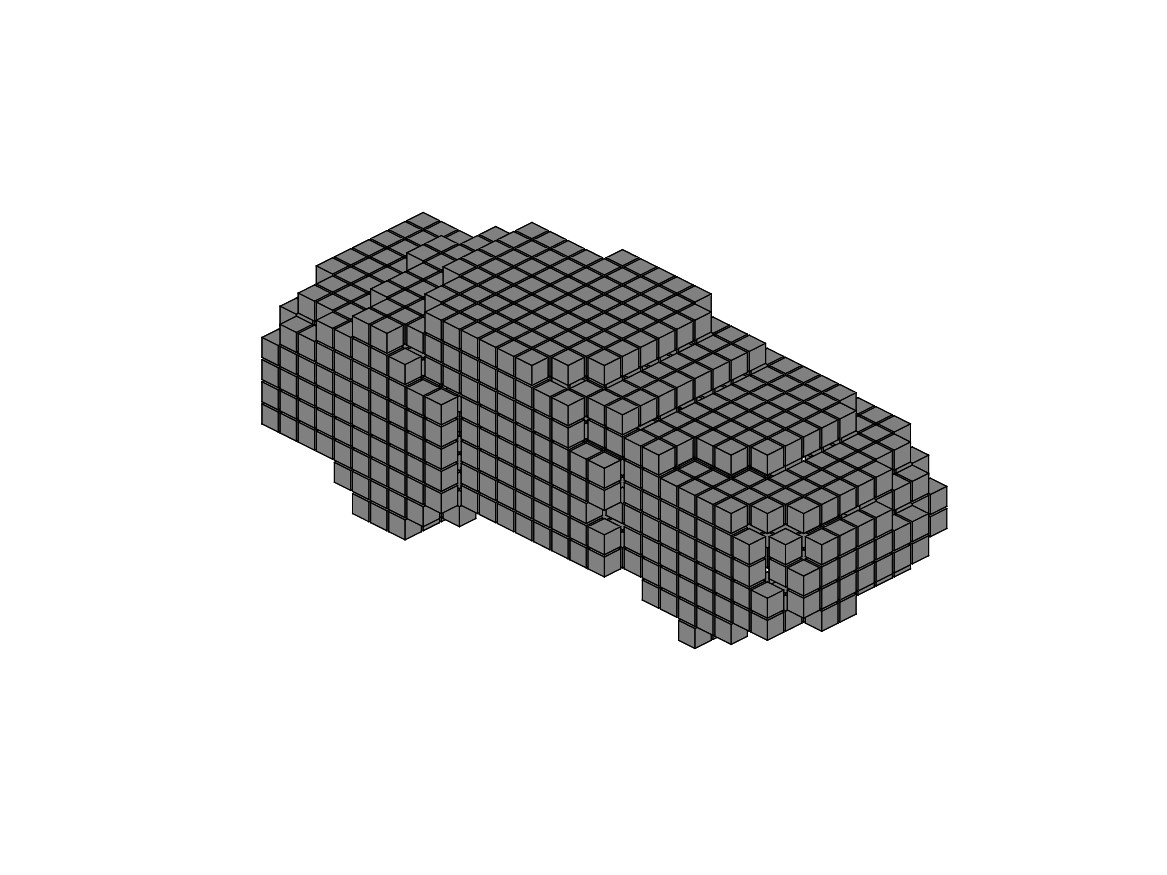
\includegraphics[width=3.75cm,trim={3.5cm 2.5cm 3.5cm 2.5cm},clip]{experiments/shapenet/vae_occ_aml/hard_15_long_statistics_75/3_target_45}
    };
    \node at (10.5, -3) {
      \includegraphics[width=3.75cm,trim={3.5cm 2.5cm 3.5cm 2.5cm},clip]{experiments/shapenet/baseline/hard_15/3_prediction_45}
    };
    
    \node at (0, 1.75) {Input};
    \node at (3.5, 1.75) {\AML};
    \node at (7, 1.75) {Baseline};
    \node at (10.5, 1.75) {Target};
  \end{tikzpicture}
  \caption{3D visualizations for comparing \AML and the supervised baseline
  on \hard difficulty of the ShapeNet dataset. Results were obtained using occupancy
  only. As can be seen, \AML has difficulties with the roofs; additionally,
  the first example occurs to the predicted with flipped orientation as our
  ShapeNet dataset also includes flipped variants.}
  \label{fig:experiments-shapenet-aml-qual-2}
\end{figure}
\begin{figure}
  \centering
  \begin{tikzpicture}    
    \node at (-3.5,0) {
      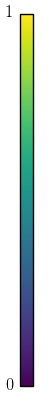
\includegraphics[height=4.25cm]{experiments/3d/vae_occ_sdf/colorbar_0}
    };
    
    \node at (0, 0){
      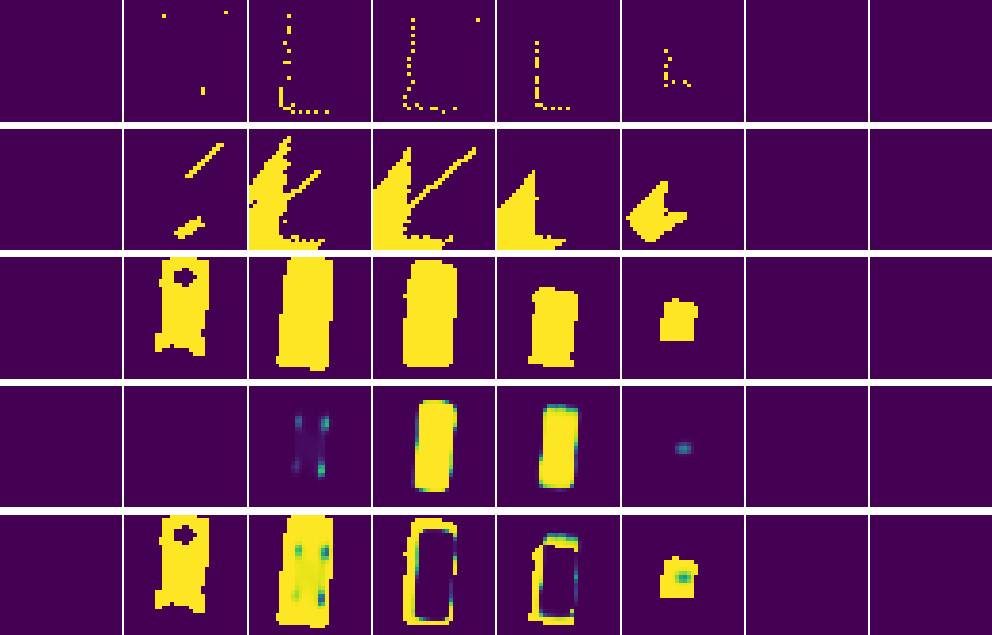
\includegraphics[width=6cm]{experiments/shapenet/vae_occ_sdf_aml/hard_15_statistics/results_0_0}
    };
    \node at (0, -4){
      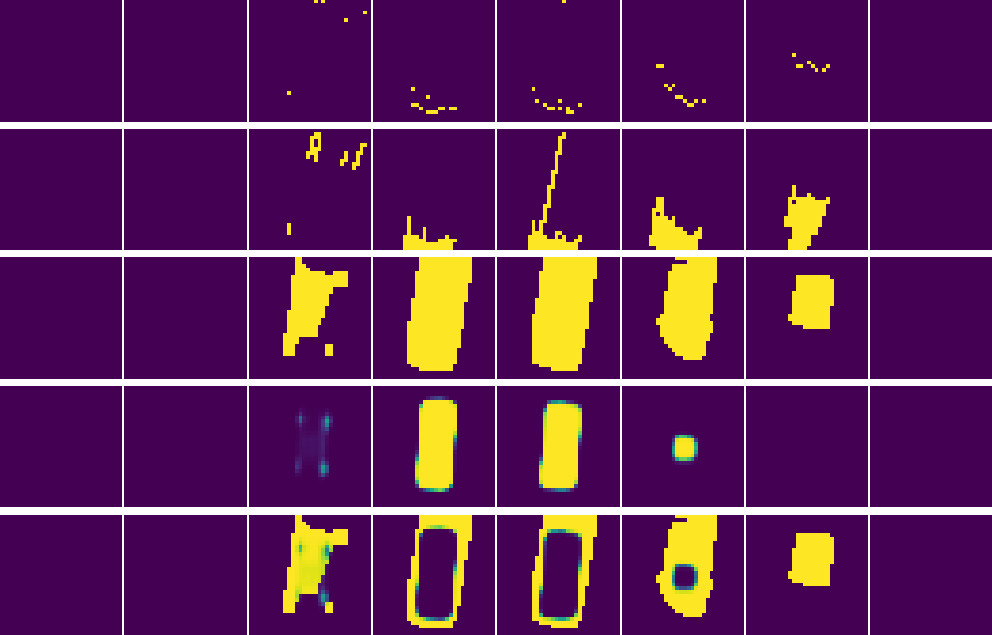
\includegraphics[width=6cm]{experiments/shapenet/vae_occ_sdf_aml/hard_15_statistics/results_3_0}
    };
    
    \node at (6.5, 0){
      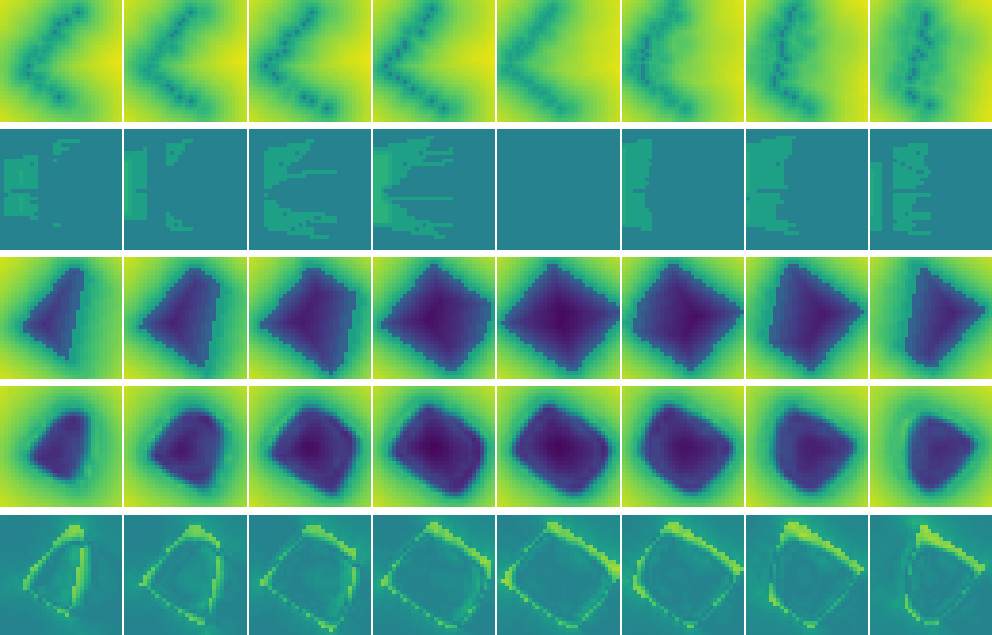
\includegraphics[width=6cm]{experiments/shapenet/vae_occ_sdf_aml/hard_15_statistics/results_0_1}
    };
    \node at (6.5, -4){
      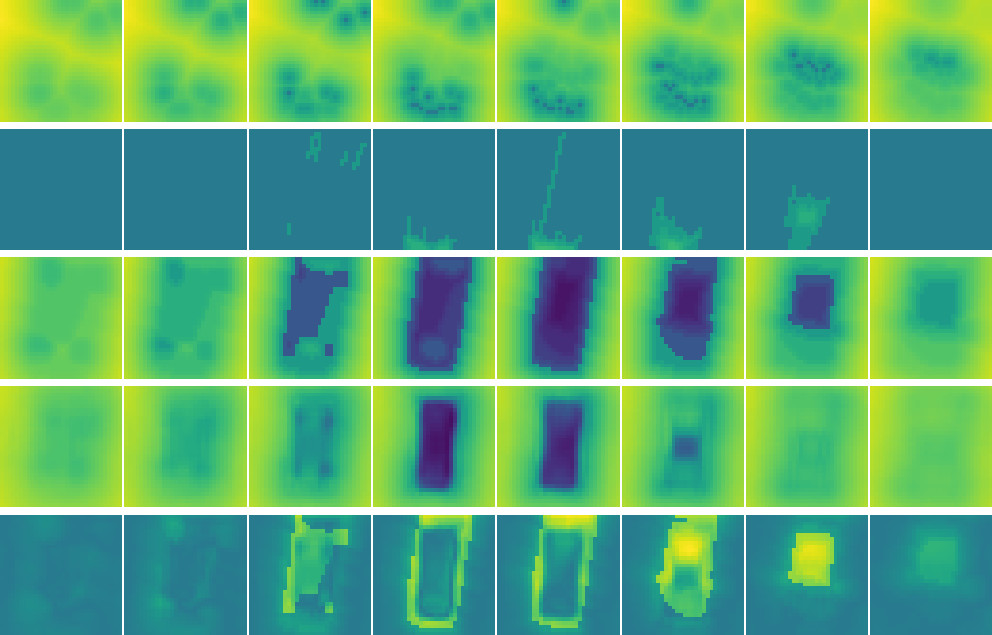
\includegraphics[width=6cm]{experiments/shapenet/vae_occ_sdf_aml/hard_15_statistics/results_3_1}
    };
    
    \node at (10,0) {
      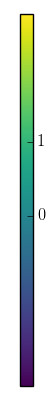
\includegraphics[height=4.25cm]{experiments/3d/vae_occ_sdf/colorbar_1}
    };
    
    \node at (0, 2.25) {occupancy};
    \node at (6.5, 2.25) {signed distance function};
  \end{tikzpicture}
  \vskip 6px

  % TODO short caption
  \caption{Qualitative results for \AML using both occupancy and signed distance
  functions. We show two examples from the \hard dataset for both modalities.
  In both cases we show slices of the volumes corresponding to the observed points,
  the partial free space, the target shape as well as the predicted shape and its
  error. Again, we show heights $8 + 2i$ for $0 \leq i < 8$. Triangular meshes
  corresponding the the predicted signed distance functions can be found
  in Figure \ref{fig:experiments-shapenet-aml-qual-4}.}
  \label{fig:experiments-shapenet-aml-qual-3}
\end{figure}
\begin{figure}
  \centering
  \begin{tikzpicture}
    \node at (0, 0) {
      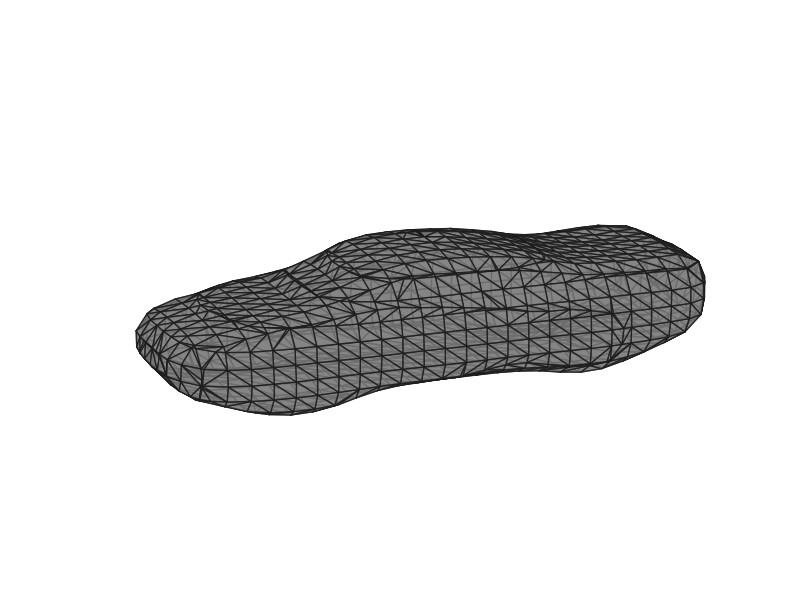
\includegraphics[width=2.75cm,trim={1cm 2cm 1cm 2cm},clip]{experiments/shapenet/vae_occ_sdf_aml/hard_15_statistics/0_prediction}
    };
    \node at (3, 0) {
      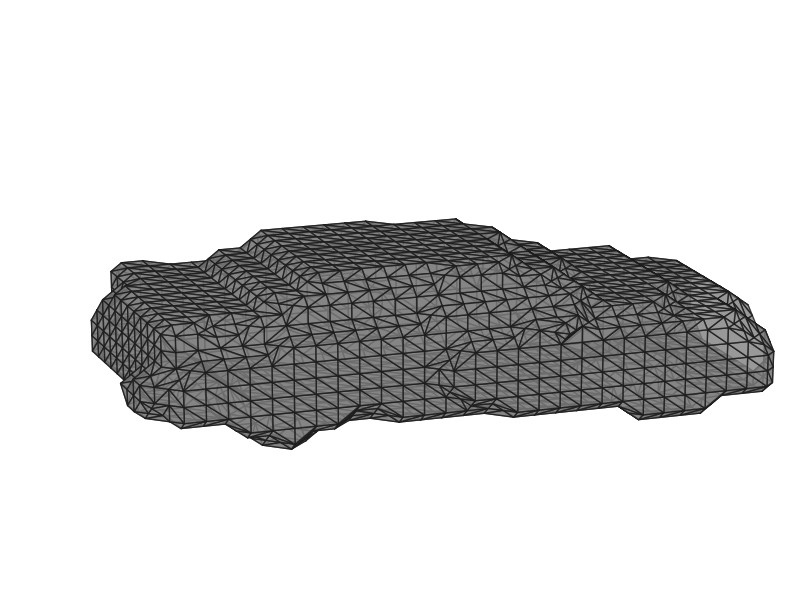
\includegraphics[width=2.75cm,trim={1cm 2cm 1cm 2cm},clip]{experiments/shapenet/vae_occ_sdf_aml/hard_15_statistics/0_target}
    };
    
    \draw[-,dashed] (5,-1) -- (5, 1);
    
    \node at (7, 0) {
      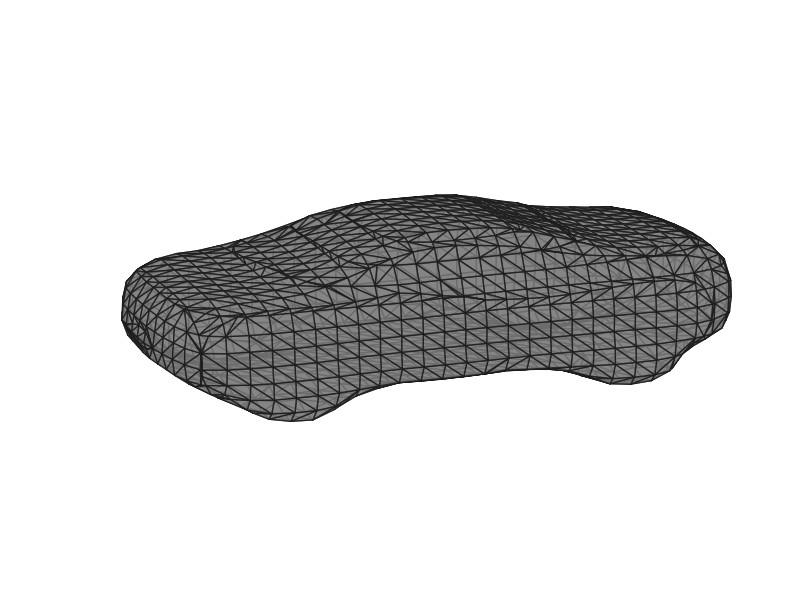
\includegraphics[width=2.75cm,trim={1cm 2cm 1cm 2cm},clip]{experiments/shapenet/vae_occ_sdf_aml/hard_15_statistics/3_prediction}
    };
    \node at (10, 0) {
      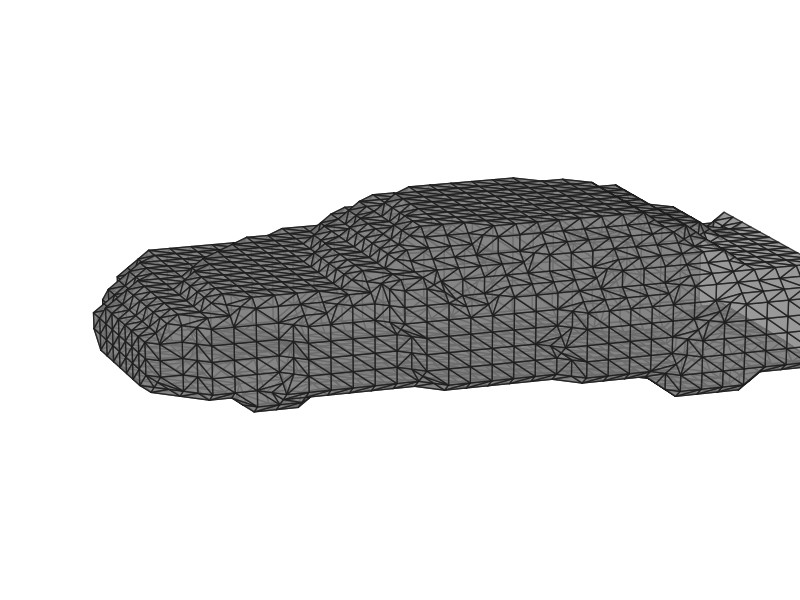
\includegraphics[width=2.75cm,trim={1cm 2cm 1cm 2cm},clip]{experiments/shapenet/vae_occ_sdf_aml/hard_15_statistics/3_target}
    };
    
    \node at (0, 1) {\AML};
    \node at (3, 1) {Target};
    \node at (7, 1) {\AML};
    \node at (10, 1) {Target};
  \end{tikzpicture}
  \caption{Qualitative results for \AML after using marchign cubes to
  derive meshes from the predictions and the targets. For the targets, we can
  clearly see that the used signed distance functions are derived from the
  occupancy grids. The predictions, in contrast a re more smooth, however,
  consistently underestimate the size of the car.}
  \label{fig:experiments-shapenet-aml-qual-4}
\end{figure}


% TODO zero error in all plots
For \AML, we follow the procedure of the 3D cuboids dataset; in Figure
\ref{fig:experiments-shapenet-aml-abs} we plot
quantitative results for the \easy, \moderate and \hard cases.
Again, it is important to keep in mind that only roughly $5.54\%$ of the voxels
are occupied. Thus, results for the \moderate and \hard cases seem quite poor:
$\Abs \approx 0.023$ and $\Abs \approx 0.027$, respectively.
This can also be observed when considering qualitative results in
Figures \ref{fig:experiments-shapenet-aml-qual-1} and
\ref{fig:experiments-shapenet-aml-qual-2} showing results for the \hard case.
We found that in many case, the predictions are very uncertain.
When considering 3D visualizations this is stressed even
more due to the thresholding. For the \moderate case, in contrast, results
look more plausible in many cases. We are not sure whether these
observations can be attributed to the prior model -- which could \eg
not be trained long enough -- or the variation in the dataset that allows
these models. It might also be beneficial to enforce the negative log-likelihood
on the prior $p(z)$ more stringent -- this assumes that the latent space
is ``more reliable'' close to $0$ than towards the tail of the Gaussian.
This could prevent shape inference from learning unlikely shapes and
potentially reduce the influence of weight initialization and stochastic
training in the first few epochs.
Overall, we see potential for improvement by tuning hyper-parameters and
longer training.

When predicting both occupancy and signed distance functions, we are not able
to achieve a performance comparable to the occupancy only case. Especially
in the \moderate and \hard cases, performance drops significantly from
$\Abs \approx 0.026$ to $\Abs \approx 0.032$ or higher (on occupancy).
We cannot say whether this is a drawback of
signed distance functions as modality, due to the shape prior or because of
the training procedure. In contrast to the occupancy only case, we did not
spend as much time tuning parameters. An exact comparison can be found in 
Figure \ref{fig:experiments-shapenet-aml-abs} while we show qualitative
results in Figures \ref{fig:experiments-shapenet-aml-qual-3}
and \ref{fig:experiments-shapenet-aml-qual-4}.
Considering the qualitative results we can, however, appreciate the
smoothing effect on the prior; the meshed predictions look very appealing -- 
in contrast to the meshed targets. Here it gets apparent that our signed
distance functions are derived from the occupancy grids. We can also
see the drop in performance; some predictions do not match the targets as
well as before; especially as \AML consistently underestimates the size
of the cars. The problems with predicting signed distance functions seem
to be consistent across datasets and models; overall, we believe that
an alternative representation might be easier to learn, \eg normalized,
discretized or just replacing the logarithm.

\subsection{Extended Variational Auto Encoder}

Although \EVAE performed slightly worse than \AML on the 3D cuboids dataset,
we still include quantitative results in Figure \ref{fig:experiments-shapenet-aml-abs}.
On ShapeNet, the performance difference between \AML and \EVAE becomes more pronounced.
However, we also want to note that, again, we did not put as much effort into
tuning parameters and training compared to \AML. Specifically, we suspect that
the weight on the Kullback-Leibler divergences may make a significant
difference. Unfortunately, we were unable to investigate this problem
further. Still, we showed, that the framework is also applicable to
real-world objects -- even if only the \easy case results in appropriate performance.
%We provide
%qualitative results in the appendix.

\subsection{Supervised Baseline}
\label{sec:experiments-shapenet-supervised-baseline}

For ShapeNet, we also prepared a supervised baseline. For a fair comparison,
we used the shape prior architecture with $Q = 15$, to learn the mapping
$x_n \mapsto y_n^*$ directly from the
synthetic data. We did not notice a significant difference between training the
exact same architecture versus removing the
Kullback-Leibler divergence and the corresponding reparameterization layer; for fairness,
we followed the former approach. We considered the \hard case only. Later,
we will also evaluate how well the learned model generalizes to KITTI.
Figure \ref{fig:experiments-shapenet-aml-abs}
shows that supervision is able to get closer to the reconstruction performance
of the shape prior, with an
absolute error of roughly $\Abs \approx 0.014$ thereby outperforming all other
presented approaches for shape completion. Qualitative results are shown in Figures
\ref{fig:experiments-shapenet-aml-qual-1} and \ref{fig:experiments-shapenet-aml-qual-2}
in comparison with \AML. Overall,
the supervised baseline could potentially also outperform \AML on KITTI, given
that the used observation model resembles KITTI's Velodyne sensor closely
enough. Overall, it is not surprising that the supervised baseline outperforms
\AML considering that \AML only uses a fraction, in particular $4.06\%$ in the
\moderate case, of the information during training.

\subsection{Discussion}

Overall, the results obtained on ShapeNet are not convincing in all cases. Especially
on \moderate and \hard difficulty, shape completion appears to be significantly
more challenging than on the 3D cuboids dataset. Unfortunately, limited time prevented us
from conducting more experiments regarding both prior and shape completion, \eg to investigate
the influence of training time, architectural changes and hyper-parameters. 
Still, the presented experiments show that the proposed approach, especially \AML
but also \EVAE in a limited setting,
are able to learn shape completion under difficult conditions.
Although we were not able to reach supervised performance, it is still surprising
what is possible under weak supervision when relying on strong shape priors.
%On KITTI,
%we also hope that a larger training set for the prior (\ie both training sets from
%Table \ref{table:experiments-shapenet-datasets}) will improve results.
We discuss possible future experiments
based on the above observations in detail in in Section \ref{sec:future-work}.
